\chapter{Controlling Weakly-coupled Carbon Spins}
\section{Carbon control (more of a theory chapter, change title) }
When on resonance (\cref{eq:res_dip_loc} ) the carbon rotates around on of two distinct anti-parallel axes based on the state the electron is in.
[Need some statement that puts the axis in the equator when on resonance. Look in appendix again ]
We define the

Figure of Bloch sphere whoing n0 and n1 axis.
A state starting of in 0 being rotated to +y and -y ($\pm $ x operation).
Different arrow


adf


Note the bloch-sphere is a model that cannot accurately represent the dynamics of a 2-qubit system. Nonetheless it can be a useful simplification in explaining qubit control. Test

More tests to see if it works

\begin{figure}[htbp]
    \begin{subfigure}[t]{0.32\textwidth}\centering
    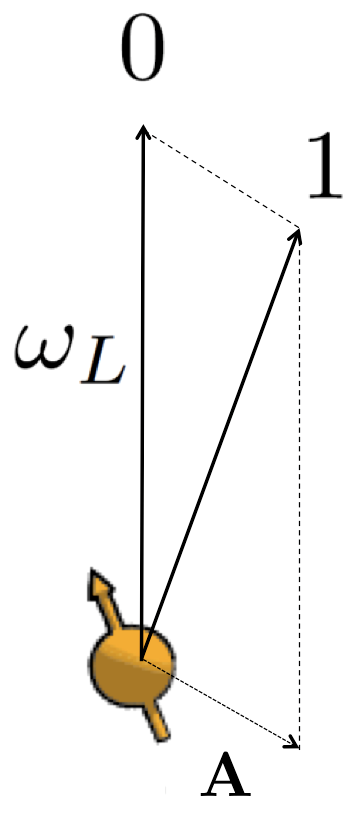
\includegraphics[scale=0.2]{Img/QuantizationAxis.png}
    \caption{Placeholder 1 }
    \end{subfigure}
    \begin{subfigure}[t]{0.32\textwidth}\centering
        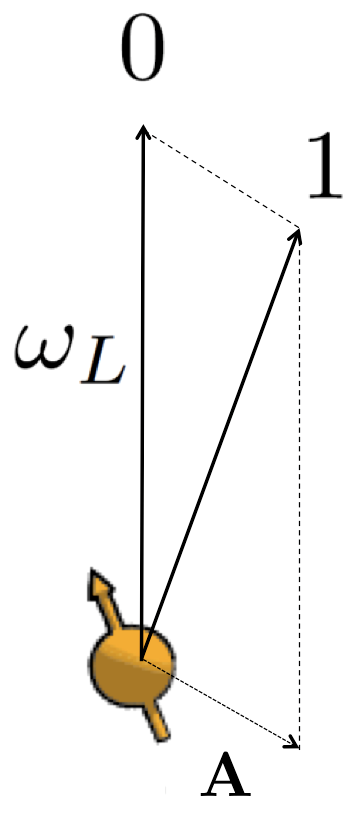
\includegraphics[scale=0.2]{Img/QuantizationAxis.png}
        \caption{Placeholder for bloch sphere }
    \end{subfigure}
    \begin{subfigure}[t]{0.32\textwidth}\centering
        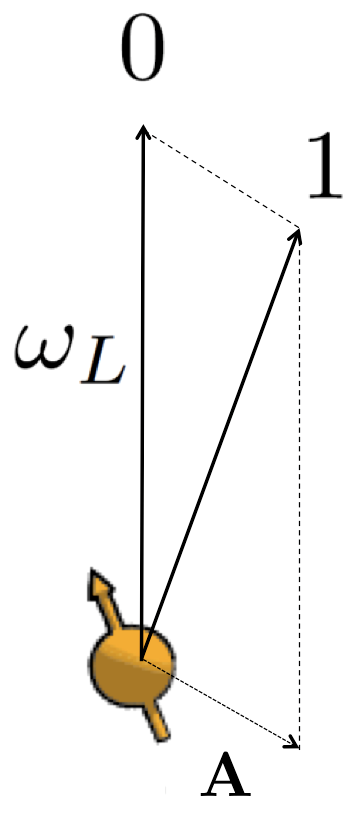
\includegraphics[scale=0.2]{Img/QuantizationAxis.png}
        \caption{Placeholder for bloch sphere }
    \end{subfigure}
    \caption{Nuclear Ramsey experiment wit}
    \label{fig:conditional_pm_x_rotation}
\end{figure}



\subsection*{Measuring Precession Frequencies}


% Ramsey experiment to measure coupling strengths
% Needs relation between frequency and parralel component
% spins 1 and 4 best



\begin{figure}[htbp]
    \centering
\mbox{
\Qcircuit @C=1em @R=.7em {
\lstick{\ket{0}}                        & \gate{\pi/2}  & \ctrl{1}      & \qw & \multigate{1}{T}       &  \qw &\ctrl{1}          & \gate{\pi/2} &\qw          &  \meter \\
\lstick{\rho_\mathrm{m}}         & \qw              &  \gate{\pm \mathrm{x}}     & \qw& \ghost{T}        & \qw & \gate{\pm \mathrm{x}}      & \qw       &\qw&
}
}
    \caption{Carbon Ramsey experiment. }
    \label{fig:gate_circuit_nuclear_ramsey}
\end{figure}


\begin{figure}[htbp]
    \begin{subfigure}[t]{0.49\textwidth}\centering
    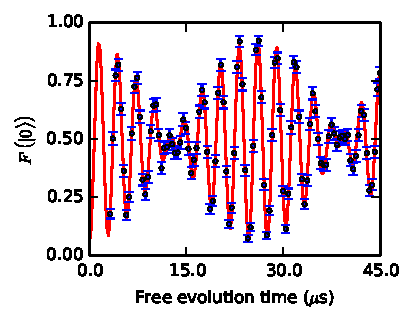
\includegraphics{Img/CarbonRamsey_C1.pdf}
    \caption{Nuclear Ramsey of Carbon 1} \label{fig:CR_C1}
    \end{subfigure}
    \begin{subfigure}[t]{0.49\textwidth}\centering
        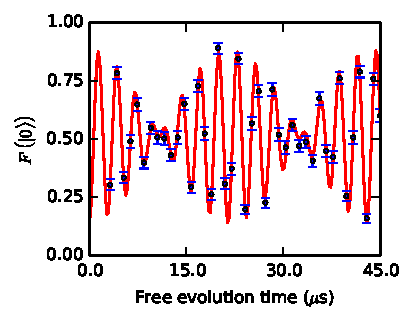
\includegraphics{Img/CarbonRamsey_C4.pdf}
        \caption{Nuclear Ramsey of Carbon 4}
        \label{fig:CR_C4}
    \end{subfigure}
    \caption{Nuclear Ramsey experiment wit}
\end{figure}



\section{Controlling weakly coupled carbons trough the electronic spin}
% Section containing theory (Gate circuits) on how to initialize and readout carbons

Explain how carbon control works in theory.
Explain how a conditional and unconditional gate can be performed.
Explain initialization on gate level, refer to appendix for calculations.
Explain Readout.



\section{Carbon Initialization \& Readout}
% TODO_MAR: Discuss naming of sec: Carbon Init&RO and Carbon Tomo
%  Section containing experimental results (Tomographies)
%  Should emphasize difficulty in seperating initialization and RO fidelity, what is not working? Is it working?
Show results that demonstrate carbon control.



